\begin{definition}
    An annuity is a finite number \(n\) of payments all of which are the same value \(R\) to be paid at a fixed period of time (e.g monthly or annually). The number of payments is called the \emph{term} and the fixed period of time is called the \emph{payment period}.
\end{definition}

Note: Since the payment period is fixed, the term can either be thought of as number of payments or measurement of time.

\begin{example}\label{rentAnn}
    A year long lease for an apartment with \(\$1250\) in rent due on the first of each month is an annuity. So, there will be \(n=12\) payments all of the same value \(R=1250.\) The payment period is \(1\) month since the rent is paid monthly. The term is \(12\) since that is the number of payments made for the year long lease. 
\end{example}

\begin{example}\label{bnplAnn}
    Common ``buy now, pay later'' services offered by online retailers represent an annuity. A typical structure might be that you pay for the total cost of goods in \(4\) payments that occur every \(2\) weeks. In this case the term is \(n=4\) and the payment period is \(2\) weeks.
\end{example}

\begin{example}\label{salaryAnn}
    Monthly payments for salaried employees represent an annuity. There is a fixed monthly or biweekly payment for \(12\) months.
\end{example}

\begin{figure}
\centering
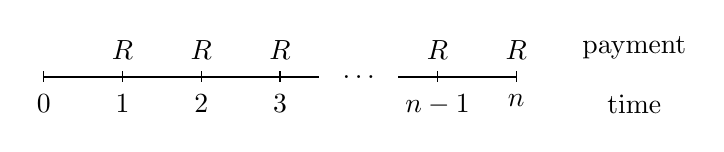
\begin{tikzpicture}
    \draw[-] (0, 0) -- (3.5, 0);
    \foreach \x in {0,1,2,3,5,6}
        \draw (\x,2pt) -- (\x,-2pt);
    \foreach \x in {1,2,3,5,6}
        \node[above] at (\x,0.1) {$R$};
    \node[below] at (0, -0.1) {$0$};
    \node[below] at (1, -0.1) {$1$};
    \node[below] at (2, -0.1) {$2$};
    \node[below] at (3, -0.1) {$3$};
    \node[below] at (5, -0.1) {$n-1$};
    \node[below] at (6, -0.1) {$n$};
    \node at (4, 0) {$\dots$};
    \draw[-] (4.5,0) -- (6,0);
    \node[above] at (7.5,0.1) {payment};
    \node[below] at (7.5, -0.1) {time};

    \end{tikzpicture}
    \caption{An illustration of the regularly scheduled fixed payments of an annuity}
    \label{ordAnn}
\end{figure}

The annuity illustrated in \autoref{ordAnn} is called an \emph{ordinary annuity} because the first payment is to be made at the \emph{end} of the first payment period. Successive payments are always made at the end of a payment period. There is also an \emph{annuity due} wherein the first payment is due immediately and the successive payments are due at the beginning of each payment period. The mathematics of each is the same beyond a shift in the time axis and so we will only cover mathematical examples of ordinary annuities. Examples \ref{rentAnn} and \ref{bnplAnn} are annuities due since those payments occur at the beginning of each pay period and Example \ref{salaryAnn} is an ordinary annuity.